\chapter{Bayesian Hyper-Heuristic}
\label{chap:bhh}

\begin{quote}
    \textit{
    The result is a ``posterior distribution'' which the agent may use as its new prior in the next step. - Pedro Domingos, The Master Algorithm: How the Quest for the Ultimate Learning Machine Will Remake Our World.
    }
\end{quote}
% \resizebox{\textwidth}{!}{
% Table generated by Excel2LaTeX from sheet 'results'
\begin{table}[htbp]
  \centering
  \caption{Add caption}
  \resizebox{\textwidth}{!}{
    % Table generated by Excel2LaTeX from sheet 'results'
    \begin{tabular}{rcccccccccc}
          & \multicolumn{10}{l}{\textbf{burn\_in}} \\
\cmidrule{2-11}          & \multicolumn{2}{l}{\textbf{0}} & \multicolumn{2}{l}{\textbf{5}} & \multicolumn{2}{l}{\textbf{10}} & \multicolumn{2}{l}{\textbf{15}} & \multicolumn{2}{l}{\textbf{20}} \\
\cmidrule{2-11}    \textbf{dataset} & \textbf{avg} & \textbf{std} & \textbf{avg} & \textbf{std} & \textbf{avg} & \textbf{std} & \textbf{avg} & \textbf{std} & \textbf{avg} & \textbf{std} \\
    \midrule
    abalone & 2.915 & 1.395 & \textbf{2.694} & 1.393 & 2.917 & 1.384 & 2.840 & 1.352 & 3.634 & 1.357 \\
    adult & 1.846 & 0.794 & 1.809 & 0.751 & 2.026 & 0.842 & \textbf{0.000} & 0.000 & \textbf{0.000} & 0.000 \\
    air\_quality & 2.910 & 1.441 & \textbf{2.682} & 1.427 & 2.770 & 1.344 & 3.372 & 1.314 & 3.267 & 1.412 \\
    car   & \textbf{2.362} & 1.231 & 2.588 & 1.425 & 3.298 & 1.392 & 3.380 & 1.271 & 3.372 & 1.401 \\
    fish\_toxicity & 3.063 & 1.459 & \textbf{2.794} & 1.402 & 2.820 & 1.513 & 3.102 & 1.346 & 3.220 & 1.295 \\
    forest\_fires & \textbf{2.816} & 1.330 & 2.849 & 1.383 & 2.865 & 1.409 & 3.377 & 1.398 & 3.092 & 1.471 \\
    housing & \textbf{2.690} & 1.384 & 2.952 & 1.318 & 2.997 & 1.442 & 3.058 & 1.344 & 3.303 & 1.510 \\
    iris  & 2.947 & 1.461 & 2.972 & 1.367 & 3.190 & 1.449 & \textbf{2.771} & 1.369 & 3.119 & 1.387 \\
    mushroom & \textbf{2.206} & 1.249 & 2.938 & 1.298 & 3.161 & 1.297 & 3.144 & 1.401 & 3.523 & 1.501 \\
    parkinsons & \textbf{2.280} & 1.282 & 2.889 & 1.247 & 2.706 & 1.314 & 3.397 & 1.417 & 3.728 & 1.330 \\
    student\_performance & \textbf{2.145} & 1.205 & 2.695 & 1.403 & 3.097 & 1.352 & 3.458 & 1.354 & 3.605 & 1.231 \\
    wine\_quality & 2.970 & 1.437 & 3.011 & 1.304 & \textbf{2.663} & 1.419 & 3.125 & 1.398 & 3.231 & 1.447 \\
    \midrule
    \textbf{overall} & \textbf{2.596} & 1.373 & 2.739 & 1.357 & 2.894 & 1.397 & 3.184 & 1.379 & 3.372 & 1.412 \\
    \end{tabular}%

    }
  \label{tab:addlabel}%
\end{table}%







The above quote was the inspiration for the development of a novel \ac{HH} that uses \index{Bayesian}\textit{Bayesian} probability concepts as a selection mechanism to drive the heuristic selection process. Thus far the reader was presented with all of the necessary background information on \acp{ANN} in Chapter \ref{chap:anns}, low-level \index{Heuristic}heuristics/\index{Optimiser}optimisers in Chapter \ref{chap:heuristics}, \acp{HH} in Chapter \ref{chap:hhs}  and lastly, \index{probability theory}probability theory in Chapter \ref{chap:probability}. These elements form the fundamental components that make up the proposed \Ac{BHH}. A detailed specification on the \Ac{BHH} can now be formulated. This chapter provides the detail around the theory, concept and implementation of the \Ac{BHH} and explains how it used to train \acp{ANN}.

The remainder of the chapter is structured as follows: Section \ref{sec:bhh:overview} provides an overview of the \Ac{BHH} optimiser. Section \ref{sec:bhh:architecture} presents the general architecture, \Ac{HH} framework and the various components that make up the \index{Optimiser}optimiser. Section \ref{sec:bhh:model} discusses the models that can be optimised using the \Ac{BHH}, specifically referring to its application to training \acp{FFNN}. Section \ref{sec:bhh:entity_pool} discusses in more detail the \index{Population}population and its \index{Entity}entities, with specific detail provided on entity (local) and population (global) state and memory. Section \ref{sec:bhh:heuristic_pool} discusses the collection of low-level \index{Heuristic}heuristics, referred to as the \index{Heuristic}Heuristic Pool and puts emphasis on the importance of a diverse set of low-level \index{Heuristic}heuristics. Section \ref{sec:bhh:performance_log} presents the performance log and discusses performance measurement in more detail. Section \ref{sec:bhh:selection_mechanism} presents the \index{Bayesian}\textit{Bayesian} probabilistic model that is used as a selection mechanism . Section \ref{sec:bhh:optimisation} presents the mechanisms by which the probabilistic model can be optimised. Section \ref{sec:bhh:hyper_parameters} summarises and discusses the associated \index{Hyper-Parameters}hyper-parameters and default values. Section \ref{sec:bhh:initialisation} presents the initialisation step in detail and Section \ref{sec:bhh:heuristic} presents the \index{Heuristic}heuristic/update step in detail. The pseudo-code algorithm is given in Section \ref{sec:bhh:algorithm} and the chapter is concluded in Section \ref{sec:bhh:conclusion}.


\section{Overview}
\label{sec:bhh:overview}

This section provides an overview of the workings of the \Ac{BHH}. To start the discussion, consider the following analogy:
\\

\textit{
    Bob is a teacher at a high school. Every year his students perform really well and he wins the prize for best teacher, evaluated by student performance. He is able to do this not just because he is a good teacher, but he understands that each student has a learning technique that works best for him/her. He exploits this concept by tailoring the teaching process to each students such that the result is an optimum mark for that student and by definition, the whole class. Bob knows that it is too timely to get to know each student, so he devises a model that does the allocations for him. This model uses a process of observation. With each evaluation opportunity he experiments by allocating different learning techniques to different students. He evaluates the student for the given opportunity and keeps a log of which learning technique he assigned to the student as well as the outcome. With each evaluation opportunity he updates his model by biasing the assignment process such that students generally get assigned learning techniques that yield the best performance for them.
}\\

The key take-out from the analogy above is the concept that Bob can maximise student performance by updating his beliefs, over time, about which learning technique to assign to which student. He does this by biasing selection/assignment towards the best combinations of student, learning technique
and evaluation opportunity. This is the basic nature of the \Ac{BHH}. The students are analogous to a population of entities. The learning techniques are analogous to heuristics/optimisers. Evaluation opportunities are analogous to time/steps/batches or even problems  and student performance is analogous to model optimisation and performance. Selecting the correct heuristic/optimiser for each entity at each optimisation step is the goal of the \Ac{BHH}. It is shown throughout this chapter that the \Ac{BHH} implements a probabilistic optimisation technique that biases a \index{Gaussian Process}\textit{Gaussian Process} (as described in Chapter \ref{chap:probability}) towards good optimisation and performance.

Formal classification of the \Ac{BHH} is needed. The authors propose classification of the \Ac{BHH} as a \textit{selective-perturbative population-based meta-\index{Hyper-Heuristic}hyper-heuristic}. The breakdown of this classification is argued as follows:

\begin{itemize}
    \item \textbf{Selective-Perturbative:} Following the classification as proposed by Burke et al. \cite{ref:burke:2010} - \textit{Selective}, meaning it has a \index{Heuristic}heuristic selection mechanism that selects from a collection of lower level \index{Heuristic}heuristics' (\index{Heuristic Pool}heuristic pool). \textit{Perturbative} - refers to its ability to combined and/or amended \index{Heuristic}heuristics update steps through a process called \textit{proxying} as will be describe later in this chapter.
    \item \textbf{Population-based:} Follows a population-based approach where a number of different \index{Candidate Solution}candidate solutions, referred to as \index{Entity}\textit{entities} work together to yield a global best solution. There is also the concept of a shared global state or memory.
    \item \textbf{Meta:} Incorporates classical, analytical and  gradient-based low level \index{Heuristic}heuristics (typically from the \ac{ML} research space) as well as meta-heuristics such as other population-based \index{Meta-Heuristic}meta-heuristics (typically from the \ac{CI} and \ac{EC} research spaces) .
    \item \textbf{Hyper-Heuristic:} Searches through the heuristic space while lower level heuristics search through the solution space.
\end{itemize}

More detailed consideration of these elements are required. The following sections break down the \Ac{BHH} into its various parts, starting with a discussion on its architecture next.


\index{Architecture}
\section{Architecture}
\label{sec:bhh:architecture}

This section aims to present the reader with all the high level components in the architecture of the \Ac{BHH}. Burke et al. \cite{ref:burke:2010} proposed an initial framework for \acp{HH} and Grobler \cite{ref:grobler:2015} further proposed a framework for a heterogeneous meta-\ac{HH}. These frameworks have been adapted for the implementation of the \Ac{BHH}. An illustration of the high-level architecture of the \Ac{BHH} is given in Figure \ref{fig:bhh_architecture} below.

\begin{figure}[H]
    \centering
    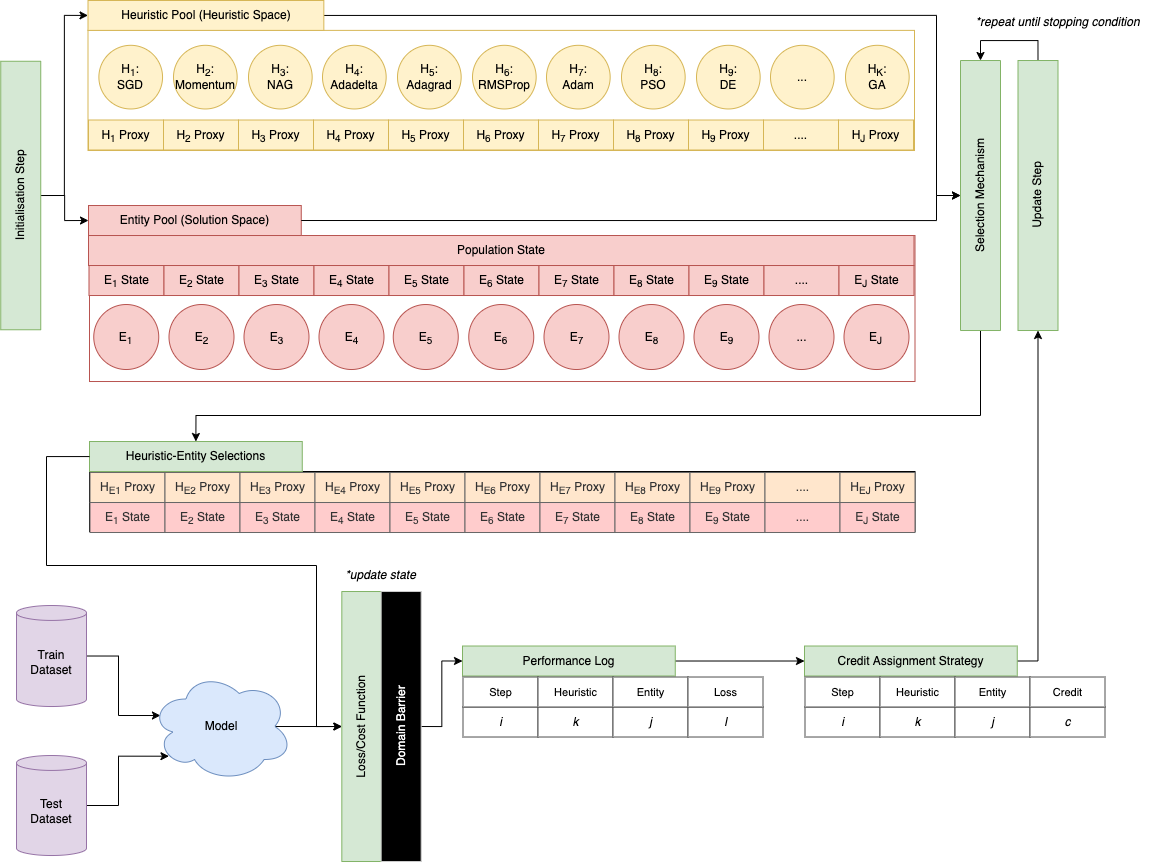
\includegraphics[width=1.0\textwidth]{bhh_architecture.png}
    \caption[The \index{Bayesian Hyper-Heuristics}Bayesian Hyper-Heuristic Architecture]{An illustration of
    the architecture and high level components of the \index{Bayesian Hyper-Heuristics}Bayesian Hyper-Heuristic.}
    \label{fig:bhh_architecture}
\end{figure}

At a high level, the architecture presented in Figure \ref{fig:bhh_architecture} above groups related elements by the following color groups:

\begin{itemize}
    \item \textbf{Purple:} Everything related to the problem domain and \index{Model}model to be optimised.
    \item \textbf{Gray:} Everything related to \index{Entity}entity (local) and shared \index{Population}population (global) state.
    \item \textbf{Red:} Everything related to \index{Entity}entities and the \index{Population}population. This also marks the components that relay information from the \index{Solution Space}\textit{solution} space.
    \item \textbf{Black:} This is the \index{Domain Barrier}domain barrier, similar to what is presented in Burke et al.'s \cite{ref:burke:2010} framework. It is a constraint on information flow, prohibiting high level components from interacting and relaying information related to the \index{Solution Space}\textit{solution} space.
    \item \textbf{Green:} Various components and strategies. These components form the main processing pipeline of the \Ac{BHH}.
    \item \textbf{Blue:} Operations performed by the \Ac{BHH}. These are complimentary operations to the processing pipeline.
    \item \textbf{Orange:} Everything related to low level \index{Heuristic}heuristics/\index{Optimiser}optimisers. This also marks the components that form part of the \index{Heuristic Space}\textit{heuristic} space.
\end{itemize}

The above grouping are not detailed enough to illustrate their role in the \Ac{BHH}. To ensure the proper clarity is given to each of these elements, a detailed discussion on each of these elements are presented next.

\index{Model}
\section{Model}
\label{sec:bhh:model}

The \index{Model}model refers to the target \index{Model}model to be optimised and is usually expressed as a complex mathematical function. For this thesis, the authors focused specifically on shallow \acp{FFNN} (only one hidden layer). Figure \ref{fig:shallow_ffnn} below presents such a shallow \acp{FFNN}.

\begin{figure}[H]
    \centering
    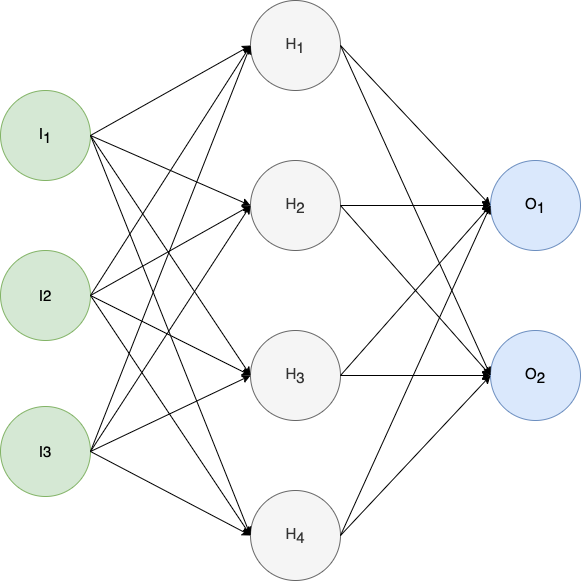
\includegraphics[width=0.4\textwidth]{shallow_ffnn.png}
    \caption[Shallow \index{Feedforward Neural Network}Feedforward Neural Network]{An illustration of
    a shallow \index{Feedforward Neural Network}Feedforward Neural Network.}
    \label{fig:shallow_ffnn}
\end{figure}

In theory, this model could take up many different forms, however one has to consider uniformity and representation, as this has an effect on the \Ac{BHH}'s design decisions:

\begin{itemize}
    \item \textbf{Uniformity:} The \index{Model}model and low-level \index{Heuristic}heuristics in the heuristic pool must be compatible. If the model is a discrete function, then only \index{Heuristic}heuristics that are applicable to discrete optimisation problems can be included.
    \item \textbf{Representation:} The \index{Model}model parameters must be presented in a manner that is compatible with low-level \index{Heuristic}heuristics. For example: a flattened 2D tensor of the model's parameters is a good, uniformly consistent representation that all lower-level heuristics can assume.
\end{itemize}

Given these two concepts above, a model is encapsulated and represented by an element known as an \index{Entity}\textit{entity}. As mentioned, the \Ac{BHH} is a \index{Population}\textit{population}-based \Ac{HH}, meaning it contains a collection of these \index{Entity}entities. Consider now a more in-depth look at the \Ac{BHH}'s entity pool.

\index{Entity Pool}
\section{Entity Pool}
\label{sec:bhh:entity_pool}

The \index{Entity Pool}\textit{entity pool} refers to a collection of so-called individual \index{Entity}\textit{entities}. A common naming convention for such a collection is a \textit{population} of entities. These \index{Entity}entities are responsible for representing a \index{Candidate Solution}candidate solution to the \index{Model}model's trainable parameters (\index{Weights}weights). These \index{Entity}entities are often  treated as physical \index{Particle}\textit{particles} in a hyper-dimensional  physical environment. This means that these \index{Entity}entities often model concepts from physics. For example, the candidate solution is represented as the \index{Entity}entity's \textit{position}. Another connection to physics is that an \index{Entity}entity's velocity and acceleration, is analogous to the gradient and momentum of an \index{Entity}entity respectfully. This concept of modeling traits of an entity as physical concept is very useful. It is later shown in Section \ref{sec:bhh:heuristic:proxies} how these concepts allows one to combine different \index{Heuristic}heuristic step operations together through a process of \index{Proxy}\textit{``proxying''}.

There are a number of parameters involved that are related to the \index{Entity Pool}entity pool/\index{Population}population and the individual \index{Entity}entities. These parameters include hyper-parameters and \textit{state} parameters .The following sections briefly discuss these concepts next.

\index{Population Size}
\subsection{Population Size}
\label{sec:bhh:entity_pool:population_size}

\index{Population Size}\textit{Population size} refers to the number of \index{Entity}entities included in the \index{Entity Pool}entity pool/\index{Population}population and is thus a \index{Hyper-Parameter}hyper-parameter of the \Ac{BHH}. The exact \index{Population Size}population size to use is problem dependent (ref ???), however in general, the larger the population the better (ref ???), assuming that entities are initialised to be spread uniformly across the solution search space. The authors propose the following considerations when picking a \index{Population Size}population size:

\begin{itemize}
    \item When considering the lower bound of possible \index{Population Size}population sizes, take into account the highest, minimum \index{Population Size}population size required by all low-level \index{Heuristic}heuristics. For example, if one includes \Ac{DE} into the \index{Heuristic}heuristic pool, one needs a \index{Population Size}population size of at least 4.
    \item When considering the upper bound of possible \index{Population Size}population sizes, take into account that the bigger the \index{Population Size}population size, the more computationally expensive it is to execute the training process. Furthermore, there exists a point of \index{Diminishing Returns}\textit{diminishing returns} where an increase in \index{Population Size}population size does not yield any better outcome (ref ???). To extend on this, consider that the \Ac{BHH} is a \Ac{HH} that utilises a \index{Bayesian}Bayesian probabilistic approach in it's selection mechanism. This means that a larger observed sample size (of entity and heuristic selection events) is needed to statistically and reliably update the selection mechanism's trainable parameters.
\end{itemize}

Following the discussion of \index{Population Size}population size is a brief discussion on a collection of stateful parameters maintained by the population as a whole, as well as individual entities as presented in the following sections.

\index{Population State}
\subsection{Population State}
\label{sec:bhh:entity_pool:population_state}

The \index{Population State}\textit{population state} refers to a collection of stateful (persisted between iterations) parameters that are shared between the \index{Entity}entities in the population. Because the \index{Population State}population state is shared between \index{Entity}entities, this state is also referred to as \index{Global State}\textit{global} state or memory. The \index{Population State}population state contains the following stateful parameters:

\begin{itemize}
    \item \textbf{\textit{entities}}: The list of entities in the population. List size determined by \index{Population Size}population size.
    \item \textbf{\textit{ibest}} and \textbf{\textit{ibest\_loss}}: Refers to the best position and loss achieved by the population for the current iteration/step.
    \item \textbf{\textit{rbest}} and \textbf{\textit{rbest\_loss}}: Refers to the best position and loss achieved by the population for the current replay buffer/window size.
    \item \textbf{\textit{gbest}} and \textbf{\textit{gbest\_loss}}: Refers to the overall/global best position and loss achieved by the population for the entire training process.
\end{itemize}

It is clear from the discussion above that entities share this stateful information and are thus required to update this information as well. This is part of state update operations and will be discussed in more detailed later in Sections \ref{sec:bhh:heuristic} and \ref{sec:bhh:algorithm}. Consider now the stateful parameters as maintained by individual entities.


\index{Entity State}
\subsection{Entity State}
\label{sec:bhh:entity_pool:entity_state}

\index{Heuristic Pool}
\section{Heuristic Pool}
\label{sec:bhh:heuristic_pool}

Inititialisation
Step

\index{Exploration}
\index{Exploitation}
\subsection{Diversity: Exploration, Exploitation and Capability}
\label{sec:bhh:entity_pool:diversity}


\index{Performance Log}
\section{Performance Log}
\label{sec:bhh:performance_log}

\index{Performance Measurement}
\subsection{Performance Measurement}
\label{sec:bhh:performance_log:performance_measurement}

\index{Credit Assignment Strategy}
\subsection{Credit Assignment Strategy}
\label{sec:bhh:performance_log:credit_assignment_strategy}

\index{Pseudo Counts}
\subsection{Pseudo Counts}
\label{sec:bhh:performance_log:pseudo_counts}

\index{Normalisation}
\subsection{Normalisation}
\label{sec:bhh:credit_assignment_strategy:normalisation}

\index{Discounted Rewards}
\subsection{Discounted Rewards}
\label{sec:bhh:credit_assignment_strategy:discounted_rewards}

\index{Pruning}
\subsection{Pruning}
\label{sec:bhh:performance_log:pruning}

\index{Selection Mechanism}
\section{Selection Mechanism}
\label{sec:bhh:selection_mechanism}

\textbf{Setup}:

\begin{itemize}
    \item $I$
    \item $J$
    \item $K$
    \item $L$

    \item $\alpha = (\alpha_{1}, \dots, \alpha_{K})$
    \item $\beta = (\beta_{1,1}, \dots, \beta_{J, K})$
    \item $\gamma = (\gamma_{1,1}, \dots, \gamma_{L, K})$

    \item $\theta \vert \alpha \sim Dir(\theta; K, \alpha)$
    \item $\phi \vert \beta \sim Dir(\phi; K, \beta)^{J}$
    \item $\psi \vert \gamma  \sim Beta(\psi; \gamma_{1}, \gamma_{2})$

    \item $H \vert \theta \sim Mult(I, H; \theta)$
    \item $E_{j} \vert \phi \sim Mult(I, H; \phi)^{J}$
    \item $C \vert \psi \sim Bin(I, \psi)$
\end{itemize}

\index{Random Events}
\subsubsection{Random Events}
\label{sec:bhh:selection_mechanism:random_events}


\index{Independence}
\subsubsection{Independence}
\label{sec:bhh:selection_mechanism:independence}

\index{Bayes' Theorem}
\subsubsection{Bayes' Theorem}
\label{sec:bhh:selection_mechanism:bayes_theorem}

The predictive model by Bayes rule:

\begin{equation}
    \begin{split}
        P(H \vert E, C;  \theta, \phi, \psi)
        &= \frac{
            P(E, C \vert H;  \phi, \psi)  P(H \vert \theta)
            }{
            P(E, C | \theta, \phi, \psi)
        } \\		
        &= \frac{
            P(E \vert H;  \phi)  P(C \vert H;  \psi) P(H \vert \theta)
            }{
            P(E | \theta, \psi) P(C | \theta, \phi)
        } \\
        &= \frac{
            P(E \vert H;  \phi)  P(C \vert H;  \psi) P(H \vert \theta)
            }{
            \left[ \sum_{k}^{K} P(E, H=k | \theta, \psi) \right] \left[ \sum_{k}^{K}  P(C, H=k | \theta, \phi) \right]
        } \\
        &= \frac{
            P(E \vert H;  \phi)  P(C \vert H;  \psi) P(H \vert \theta)
            }{
            \left[ \sum_{k}^{K} P(E | H=k | \phi) P(H=k \vert \theta) \right] \left[ \sum_{k}^{K} P(C | H=k | \psi) P(H=k \vert \theta) \right]
        }
    \end{split}
\end{equation}

One should start to notice the joint probability over events $E$ and $C$ given the selection of a heuristic $H$ denoted by the sums of the products of the separate parts, for $E$ and $C$, in the denominator.

In order to derive the posterior distribution as given in Equestion (ref?? above), one only has to evaluate to proportionality as follows:

\begin{equation}
    \begin{split}
        P(H \vert E, C;  \theta, \phi, \psi) &\propto P(E \vert H;  \phi)  P(C \vert H;  \psi) P(H \vert \theta)
    \end{split}
\end{equation}


\index{Naïve Bayes}
\subsubsection{Naïve Bayes}
\label{sec:bhh:selection_mechanism:naive_bayes}

One very big assumption that is made by the Naïve Bayes Classifier is that it
assumes that all features are conditionally independent given the class label
(ref ??). \\
The independence between events for the class label $H$ simply yields the PMF of the Multinomial distribution as follows:

\begin{equation}
    \begin{split}
        P(H \vert \theta)
        &\propto \prod_{i=1}^{I} \prod_{k=1}^{K} P(h_{i,k} \vert \theta_{k}) \\
        &\propto \prod_{i=1}^{I} \prod_{k=1}^{K} \theta_{k}^{\mathbbm{1}_{1}(h_{i,k})} \\
        &\propto \prod_{k=1}^{K} \theta_{k}^{\sum_{i=1}^{I} \mathbbm{1}_{1}(h_{i,k})} \\
        &\propto \prod_{k=1}^{K} \theta_{k}^{N_{k}}
    \end{split}
\end{equation}

where $N_{k}$ is a summary variable such that $N_{k} = \sum_{i=i}^{I}
\mathbbm{1}_{1}(h_{i,k})$, denoting the count of occurrences of the event
$h_{i}$ taking on class $k$, i.e. the count of occurrences of heuristic $k$ in
$I$ independent, identical runs.\\ The independence between events for the
entities feature $E$ given class label $H$ is denoted by the likelihood of $E$
conditional to the occurrence of heuristic $k$ and model parameter $\phi$ as
follows:

\begin{equation}
    \begin{split}
        P(E \vert H;  \phi)
        &\propto \prod_{i=1}^{I} \prod_{j=1}^{J} \prod_{k=1}^{K} P(e_{i,j,k} \vert h_{i,k} ; \phi_{j,k})  \\
        &\propto \prod_{i=1}^{I} \prod_{j=1}^{J} \prod_{k=1}^{K} \phi_{j,k}^{\mathbbm{1}_{1}(e_{i,j,k})\mathbbm{1}_{1}(h_{i,k})} \\
        &\propto \prod_{j=1}^{J} \prod_{k=1}^{K} \phi_{j,k}^{ \sum_{i}^{I} \left[ \mathbbm{1}_{1}(e_{i,j,k}) \mathbbm{1}_{1}(h_{i,k}) \right]} \\
        &\propto \prod_{j=1}^{J} \prod_{k=1}^{K} \phi_{j,k}^{N_{j,k}}
    \end{split}
\end{equation}

where $N_{j,k}$ is a summary variable such that $N_{j,k} = \sum_{i=i}^{I}
\mathbbm{1}_{1}(e_{i,j,k})\mathbbm{1}_{1}(h_{i,k})$, denoting the count of
occurrences of the events $e_{i}$ taking on class $j$ and $h_{i}$ taking on
class $k$, i.e. the count of occurrences of both entity entity $e$ and heuristic
$k$ occurring together in $I$ independent, identical runs.\\ Finally, the
independence between events for the performance criteria feature $C$ given class
label $H$ is denoted by the likelihood of $C$ conditional to the occurrence of
heuristic $k$ and model parameter $\psi$ as follows:

\begin{equation}
    \begin{split}
        P(C\vert H;  \psi)
        &\propto\prod_{i=1}^{I} \prod_{k=1}^{K} P(c_{i,k} \vert h_{i,k} ; \psi_{k})  \\
        &\propto \prod_{i=1}^{I} \prod_{k=1}^{K} \psi_{k}^{\mathbbm{1}_{1}(c_{i,k})\mathbbm{1}_{1}(h_{i,k})} (1 - \psi_{k})^{\mathbbm{1}_{0}(c_{i,k})\mathbbm{1}_{1}(h_{i,k})}\\
        &\propto \prod_{k=1}^{K} \psi_{k}^{\sum_{i=1}^{I} \mathbbm{1}_{1}(c_{i,k})\mathbbm{1}_{1}(h_{i,k})} (1 - \psi_{k})^{\sum_{i=1}^{I} \mathbbm{1}_{0}(c_{i,k})\mathbbm{1}_{1}(h_{i,k})}\\
        &\propto \prod_{k=1}^{K} \psi_{k}^{N_{1,k}} (1 - \psi_{k})^{N_{0,k}} \\
        &\propto \prod_{k=1}^{K} \psi_{k}^{N_{1,k}} (1 - \psi_{k})^{(N_{k} - N_{1,k})}
    \end{split}
\end{equation}

where $N_{k}$ is the summary variable as described for Equation (ref ??) above.
$N_{1,k}$ is a summary variable such that $N_{1,k} = \sum_{i=1}^{I}
\mathbbm{1}_{1}(c_{i,k})\mathbbm{1}_{1}(h_{i,k})$, denoting the count of
occurrences of the events $c_{i}$ taking on a success $(c_{i}=1)$ and $h_{i}$
taking on class $k$, i.e. the count of occurrences of both succeeding in the
performance criteria and heuristic $k$ occurring together in $I$ independent,
identical runs. Similarly $N_{0,k} = N_{k} - N_{1,k}$ would denote the count of
occurrences of the events $c_{i}$ taking on a failure $(c_{i}=0)$ and $h_{i}$
taking on class $k$. \\
By the assumptions made by the Naïve Bayes Classifier, one could supplement
Equations (ref ??, ??, ??) above into the proportional evaluation of the
predictive model as given in Equation (ref ??) as follows:

\begin{equation}
    \begin{split}
        P(H \vert E, C;  \theta, \phi, \psi)
    &\propto P(E \vert H;  \phi)  P(C \vert H;  \psi) P(H \vert \theta)  \\
    &\propto \left[ \prod_{j=1}^{J} \prod_{k=1}^{K} \phi_{j,k}^{N_{j,k}} \right] \left[ \prod_{k=1}^{K} \psi_{k}^{N_{1,k}} (1 - \psi_{k})^{(N_{k} - N_{1,k})} \right] \left[ \prod_{k=1}^{K} \theta_{k}^{N_{k}} \right]
    \end{split}
\end{equation}


\index{Numerical Stability}
\subsubsection{Numerical Stability}
\label{sec:bhh:selection_mechanism:numerical_stability}

\index{Mode Collapse}
\subsubsection{Mode Collapse}
\label{sec:bhh:selection_mechanism:mode_collapse}

\index{Burn In}
\subsubsection{Burn In}
\label{sec:bhh:selection_mechanism:burn_in}

\index{Replay}
\subsubsection{Replay}
\label{sec:bhh:selection_mechanism:replay}

\index{Reanalysis}
\subsubsection{Reanalysis}
\label{sec:bhh:selection_mechanism:reanalysis}

\index{Reselection}
\subsubsection{Reselection}
\label{sec:bhh:selection_mechanism:reselection}



\index{Optimisation}
\section{Optimisation}
\label{sec:bhh:optimisation}

Online learning...

\index{Performance Bias}
\subsection{Performance Bias}
\label{sec:bhh:optimisation:performance_bias}


\index{A Priori Bias}
\subsection{A Priori Bias}
\label{sec:bhh:optimisation:a_priori_bias}


\index{Maximum Likelihood Estimation}
\subsection{Maximum Likelihood Estimation}
\label{sec:bhh:optimisation:mle}

By calculating the Maximum Likelihood Estimate (MLE) of $\theta$, $\phi$ and $\psi$ it can be shown that:

\begin{itemize}
    \item $\hat{\theta}_{k} = E[\theta_{k}] = \frac{N_{k}}{N}$
    \item $\hat{\phi}_{j,k} = E[\phi_{j,k}] = \frac{N_{j,k}}{N_{j}}$
    \item $\hat{\psi}_{k} = E[\psi_{k}] = \frac{N_{1,k}}{N_{k}}$
\end{itemize}

The calculations of the MLE for $\hat{\theta}_{k}$, $\hat{\phi}_{j,k}$ and
$\hat{\psi}_{k}$ is now presented.\\
The log likelihood of $\hat{\theta}$, $\hat{\phi}$ and $\hat{\psi}$ as derived
from the Equations (ref ??????) above is given as:

\begin{equation}
    \begin{split}
        & \mathcal{L}(\theta, \phi, \psi) \\
        &= \ln\left(\left[ \prod_{j=1}^{J} \prod_{k=1}^{K} \phi_{j,k}^{N_{j,k}} \right] \left[ \prod_{k=1}^{K} \psi_{k}^{N_{1,k}} (1 - \psi_{k})^{(N_{k} - N_{1,k})} \right] \left[ \prod_{k=1}^{K} \theta_{k}^{N_{k}} \right] \right) \\
        &= \ln \left( \prod_{j=1}^{J} \prod_{k=1}^{K} \phi_{j,k}^{N_{j,k}} \right) +  \ln \left( \prod_{k=1}^{K} \psi_{k}^{N_{1,k}} (1 - \psi_{k})^{(N_{k} - N_{1,k})} \right) + \ln \left( \prod_{k=1}^{K} \theta_{k}^{N_{k}} \right) \\		
        &= \left( \sum_{j=1}^{J} \sum_{k=1}^{K} N_{j,k} \ ln \left( \phi_{j,k}
        \right) \right) \\
        &+ \left( \sum_{k=1}^{K} N_{1,k} \ln \left( \psi_{k} \right) + \left( N_{k} - N_{1,k} \right) \ln \left( 1 - \psi_{k} \right) \right) + \left( \sum_{k=1}^{K} N_{k} \ln \left( \theta_{k} \right) \right)
    \end{split}
\end{equation}

Consider the log likelihood of $\psi$  as denoted by:

\begin{equation}
    \begin{split}
        \mathcal{L}(\psi) &=  \sum_{k=1}^{K} N_{1,k} \ln \left( \psi_{k} \right) + \left( N_{k} - N_{1,k} \right) \ln \left( 1 - \psi_{k} \right)
    \end{split}
\end{equation}

The MLE for $\hat{\psi_{k}} $ can be calculated by taking the derivative of Equation (ref ?? above) with respect to $\psi_{k}$ and equating to zero as follows:

\begin{equation}
    \begin{split}
        \frac{\partial \mathcal{L}(\psi)}{\partial \psi_{k}} &= N_{1,k} \frac{1}{ \psi_{k}} + \left( N_{k} - N_{1,k} \right) \frac{-1}{ \left( 1 - \psi_{k} \right) } \\
        0 &=  \frac{ N_{1,k} \left( 1 - \psi_{k} \right) +  \left( N_{1,k} - N_{k} \right) \psi_{k}}{ \psi_{k} \left( 1 - \psi_{k} \right) } \\
        0 &=  N_{1,k} \left( 1 - \psi_{k} \right) +  \left( N_{1,k} - N_{k} \right) \psi_{k} \\
        0 &=  N_{1,k} - N_{1,k} \psi_{k}  +  N_{1,k} \psi_{k} - N_{k}\psi_{k} \\
        0 &=  N_{1,k} - N_{k}\psi_{k} \\
        N_{k}\psi_{k} &=  N_{1,k} \\
        \hat{\psi}_{k} &=  \frac{N_{1,k}}{N_{k}} \\
    \end{split}
\end{equation}


The value for $\hat{\theta_{k}} $ can be calculated similarly. However, one has to compensate for the $K-1$ Simplex $S$ by adding error factor $\epsilon$ to correct values for  $\theta$ where $\sum_{k}^{K} \theta_{k} \neq 1$. The new log likelihood function is then:

\begin{equation}
    \begin{split}
        \mathcal{L}(\theta, \epsilon)
        &=  \left( \sum_{k=1}^{K} N_{k} \ln \left( \theta_{k} \right) \right) + \epsilon \left( 1 - \sum_{k=1}^{K} \theta_{k} \right) \\
        &=  \left( \sum_{k=1}^{K} N_{k} \ln \left( \theta_{k} \right) \right) + \left( \epsilon -  \epsilon \sum_{k=1}^{K} \theta_{k} \right)
    \end{split}
\end{equation}

Solving first for $\epsilon$:

\begin{equation}
    \begin{split}
        \frac{\partial \mathcal{L}(\theta, \epsilon)}{\partial \epsilon} &= 1 - \sum_{k=1}^{K} \theta_{k}  \\
        \sum_{k=1}^{K} \theta_{k}  &= 1
    \end{split}
\end{equation}

then for $\theta_{k}$:

\begin{equation}
    \begin{split}
        \frac{\partial \mathcal{L}(\theta, \epsilon)}{\partial \theta_{k}} &=  N_{k} \frac{1}{\theta_{k}}  + \epsilon(-1) \\
        \frac{N_{k}}{\theta_{k}} &= \epsilon \\
        N_{k} &= \theta_{k} \epsilon \\
        \sum_{k=1}^{K} N_{k} &= \sum_{k=1}^{K} \theta_{k} \epsilon \\
        N &= \epsilon \sum_{k=1}^{K} \theta_{k} \\
        N &= \epsilon
    \end{split}
\end{equation}

Substituting back into the Equation yields:

\begin{equation}
    \begin{split}
        N_{k} &= \theta_{k} \epsilon \\
        N_{k} &= \theta_{k} N \\
        \hat{\theta}_{k} &= \frac{N_{k}}{N}\\
    \end{split}
\end{equation}

The value for $\hat{\phi}_{j, k} $ is calculated very similarly. To compensate for the $K-1$ Simplex $S$ an error factor $\lambda = (\lambda_{1}, \dots, \lambda_{J})$ is added. This follows:

\begin{equation}
    \begin{split}
        \mathcal{L}(\phi, \lambda) 
        &=  \left( \sum_{j=1}^{J} \sum_{k=1}^{K} N_{j,k} \ ln \left( \phi_{j,k} \right) \right) + \sum_{j=1}^{J} \lambda_{j} \left( 1 - \sum_{k=1}^{K} \phi_{j,k} \right) \\
        &=  \left( \sum_{j=1}^{J} \sum_{k=1}^{K} N_{j,k} \ ln \left( \phi_{j,k} \right) \right) + \sum_{j=1}^{J} \lambda_{j} - \sum_{j=1}^{J} \lambda_{j} \sum_{k=1}^{K} \phi_{j,k} \\
    \end{split}
\end{equation}

Solving first for $\lambda_{j}$:

\begin{equation}
    \begin{split}
        \frac{\partial \mathcal{L}(\phi, \lambda)}{\partial \lambda_{j}} &= 1 - \sum_{k=1}^{K} \phi_{j,k}  \\
        \sum_{k=1}^{K} \phi_{j,k}  &= 1
    \end{split}
\end{equation}

then for $\phi_{j,k}$:

\begin{equation}
    \begin{split}
        \frac{\partial \mathcal{L}(\phi, \lambda)}{\partial \phi_{j,k}} &= N_{j,k} \frac{1}{\phi_{j,k}}  - \lambda_{j} \\
        \frac{N_{j,k}}{\phi_{jk}} &= \lambda_{j} \\
        N_{j,k} &= \phi_{j,k} \lambda_{j} \\
        \sum_{k=1}^{K} N_{j,k} &= \sum_{k=1}^{K} \phi_{j,k} \lambda_{j} \\
        N_{j} &= \lambda_{j} \sum_{k=1}^{K} \phi_{j,k} \\
        N_{j} &= \lambda_{j}
    \end{split}
\end{equation}

Substituting back into the Equation yields:

\begin{equation}
    \begin{split}
        N_{j,k} &= \phi_{j,k} \lambda_{j} \\
        N_{j,k} &= \phi_{j,k} N_{j} \\
        \hat{\phi}_{j,k} &= \frac{N_{j,k}}{N_{j}}\\
    \end{split}
\end{equation}

\index{Maximum a Posteriori Estimation}
\subsection{Maximum a Posteriori Estimation}
\label{sec:bhh:optimisation:map}

I.e. Bayesian Analysis

Another approach to optimising the values for $\hat{\theta}_{k}$, $\hat{\phi}_{j,k}$ and $\hat{\psi}_{k}$ is to optimise the parameters to their probability distributions. This process is referred to as Bayesian Analysis. This process is of particular importance to this paper as it is used to sample the probabilities of heuristic selection in the selection mechanism to the Bayesian Hyper Heuristic. The detail of this application is described in Chapter (ref??? this chapter).

Bayesian Analysis makes use of the posterior probability distribution. The posterior distribution is simply expressed as:

\begin{equation*}
    \begin{split}
        POSTERIOR \propto LIKELIHOOD \times PRIOR
    \end{split}
\end{equation*}

The likelihood is presented in Equation (ref ???) above. The event $H$ is a multinomial distribution with parameter $\theta$ and from Chapter (ref ?? maybe this chapter) it is known that the prior to a multinomial distribution is a Dirichlet distribution. The prior for $\hat{\theta}_{k}$ is thus presented in Equation (ref??) below:

\begin{equation}
    \begin{split}
        P(\theta | \alpha)
&\propto \prod_{k=1}^{K} \theta_{k}^{\alpha_{k} -1}
    \end{split}
\end{equation}

Furthermore, the event $E$ is also multinomial distribution with parameter $\phi$. The prior for $\hat{\phi}_{j,k}$ is thus presented in Equation (ref??) below:

\begin{equation}
    \begin{split}
        P(\phi | \beta)
&\propto \prod_{j=1}^{J}  \prod_{k=1}^{K} \phi_{j,k}^{\beta_{j,k} -1}
    \end{split}
\end{equation}

Finally,  the event $C$ is a binomial distribution with parameter $\psi$ and from Chapter (ref ?? maybe this chapter) it is known that the prior to a binomial distribution is a Beta distribution. The prior for $\hat{\psi}_{k}$ is thus presented in Equation (ref??) below:

\begin{equation}
    \begin{split}
        P(\psi | \gamma_{1}, \gamma_{2})
&\propto \prod_{k=1}^{K} \psi_{k}^{\gamma_{1,k}} (1- \psi_{k})^{\gamma_{2,k}}
    \end{split}
\end{equation}

Putting the likelihood and priors together yields the posterior distribution as given in Equation (ref ??) below:

\begin{equation}
    \begin{split}
& P(\theta, \phi, \psi \vert H, E, C;  \alpha, \beta, \gamma_{1}, \gamma_{2}) \\
&\propto P(H \vert E, C; \theta, \phi, \psi)P(\theta, \phi, \psi \vert \alpha, \beta, \gamma_{1}, \gamma_{2}) \\
&\propto P(E \vert H; \phi) P(C \vert H; \psi) P(H \vert \theta) P(\phi \vert \beta) P(\psi \vert \gamma_{1}, \gamma_{2}) P(\theta \vert \alpha)  \\
&\propto \left[ \prod_{j=1}^{J} \prod_{k=1}^{K} \phi_{j,k}^{N_{j,k}} \right] \left[ \prod_{k=1}^{K} \psi_{k}^{N_{1,k}} (1 - \psi_{k})^{(N_{k} - N_{1,k})} \right] \left[ \prod_{k=1}^{K} \theta_{k}^{N_{k}} \right] \\
&\times \left[ \prod_{j=1}^{J} \prod_{k=1}^{K} \phi_{j,k}^{\beta_{j,k} - 1} \right] \left[ \prod_{k=1}^{K} \psi_{k}^{\gamma_{1,k} - 1} (1 - \psi_{k})^{\gamma_{2,k} - 1} \right] \left[ \prod_{k=1}^{K} \theta_{k}^{\alpha_{k} - 1} \right] \\
&\propto \left[ \prod_{j=1}^{J} \prod_{k=1}^{K} \phi_{j,k}^{(N_{j,k} + \beta_{j,k}) - 1} \right] \\
&\times \left[ \prod_{k=1}^{K} \psi_{k}^{(N_{1,k} + \gamma_{1,k}) - 1} (1 - \psi_{k})^{(N_{0,k} + \gamma_{2,k} )- 1} \right] \\
&\times \left[ \prod_{k=1}^{K} \theta_{k}^{(N_{k} + \alpha_{k}) - 1} \right]
    \end{split}
\end{equation}

From Equation (Ref ??) above, it can be seen that the posterior distribution has the same form as the prior distribution. Meaning that the parameters to the priors can by updated to:

\begin{itemize}
    \item $\alpha_{k}(t+1) = N_{k} + \alpha_{k}(t)$
    \item $\beta_{j,k}(t+1) = N_{j,k} + \beta_{j,k}(t)$
    \item $\gamma_{1,k}(t+1) = N_{1,k} + \gamma_{1,k}(t)$
    \item $\gamma_{2,k}(t+1) = N_{0,k} + \gamma_{2,k}(t)$
\end{itemize}

\index{Hyper-Parameters}
\section{Hyper-Parameters}
\label{sec:bhh:hyper_parameters}

\subsection{Defaults}
\label{sec:bhh:hyper_parameters:defaults}

\index{Initialisation}
\section{Initialisation}
\label{sec:bhh:initialisation}

\index{Heuristic}
\section{Heuristic}
\label{sec:bhh:heuristic}

\index{Proxies}
\subsection{Proxies}
\label{sec:bhh:heuristic:proxies}

\index{Momentum}
\subsection{Momentum}
\label{sec:bhh:heuristic:momentum}

\index{Algorithm}
\section{Algorithm}
\label{sec:bhh:algorithm}

% Algorithm2e comment style
\SetKwComment{Comment}{/* }{ */}
\RestyleAlgo{ruled}
\begin{algorithm}[H]
\caption{The \index{Bayesian Hyper-Heuristic} Bayesian Hyper-Heuristic Optimiser
}
\label{algo:bhh}

\KwData{$n \geq 0$}
\KwResult{$y = x^n$}

$y \gets 1$\;
$X \gets x$\;
$N \gets n$\;

\While{$N \neq 0$}{
  \eIf{$N$ is even}{
    $X \gets X \times X$\;
    $N \gets \frac{N}{2}$ \Comment*[r]{This is a comment}
  }{\If{$N$ is odd}{
      $y \gets y \times X$\;
      $N \gets N - 1$\;
    }
  }
}
\end{algorithm}


\index{Conclusion}
\section{Conclusion}
\label{sec:bhh:conclusion}

